\documentclass[conference]{IEEEtran}
\IEEEoverridecommandlockouts
% The preceding line is only needed to identify funding in the first footnote. If that is unneeded, please comment it out.
% \usepackage{cite}
% Enables Portuguese Brasil
% \usepackage[portuguese]{babel}
%encoding
\usepackage[numbers]{natbib}
% Enables code listing
\usepackage{listings}
%--------------------------------------
\usepackage[T1]{fontenc}
\usepackage[utf8]{inputenc}
%--------------------------------------
%Enables the use of greek letter without a math context
\usepackage{textgreek}
%--------------------------------------
%Enables hiperlinks
\usepackage[hidelinks]{hyperref}
%--------------------------------------

\usepackage{amsmath,amssymb,amsfonts}
\usepackage{algorithmic}
\usepackage{graphicx}
\usepackage{textcomp}
\usepackage{xcolor}

\usepackage{color, colortbl}

% The code style
\usepackage{color}
\definecolor{codegreen}{rgb}{0,0.6,0}
\definecolor{codegray}{rgb}{0.5,0.5,0.5}
\definecolor{codepurple}{rgb}{0.58,0,0.82}
\definecolor{backcolour}{rgb}{0.95,0.95,0.92}

\lstdefinestyle{mystyle}{
	backgroundcolor=\color{backcolour},   
	commentstyle=\color{codegreen},
	keywordstyle=\color{magenta},
	numberstyle=\tiny\color{codegray},
	stringstyle=\color{codepurple},
	basicstyle=\footnotesize,
	breakatwhitespace=false,         
	breaklines=true,                 
	captionpos=b,                    
	keepspaces=true,                 
	numbers=left,                    
	numbersep=2pt,                  
	showspaces=false,                
	showstringspaces=false,
	showtabs=false,                  
	tabsize=2
}
\lstset{style=mystyle}
%---------------------------------------

\def\BibTeX{{\rm B\kern-.05em{\sc i\kern-.025em b}\kern-.08em
		T\kern-.1667em\lower.7ex\hbox{E}\kern-.125emX}}

\begin{document}
	\title{A brief review of Quantum Mechanics for Computer Scientists}
	\author{André Furlan - UNESP - Universidade Estadual Paulista "Júlio de Mesquita Filho"}
	\date{2023-06-01}
	\maketitle
	
	\begin{abstract}
		Quantum computers are one of the most promising technologies currently. However, a lack of understanding of its basic concepts may hinder even experienced computer scientists from exploring its possibilities. This document aims to provide a brief review of these concepts to enable those interested in quantum computation to understand and utilize its ideas effectively. For a broader explanation of quantum computing, I recommend the insightful work "Introdução à Computação Quântica" by Wagner Jorcuvich Nunes da Silva (2018) \cite{da2018introduccao}.
	\end{abstract}
	
	\begin{IEEEkeywords}
		quantum mechanics, quantum computation, qubit
	\end{IEEEkeywords}
	
	\section{Introduction}
		\par In the same century that classical computers, with their classical bits that can only assume one of two values (0 or 1), emerged, another field of knowledge arose: Quantum Mechanics. This field was developed to explain phenomena in the microscopic domain that could not be adequately described by Newtonian mechanics. As some quantum phenomena, such as entanglement and superposition, exhibit counterintuitive behavior, scientists began exploring the possibility of utilizing these behaviors in computing, leading to the birth of quantum computing.
		
	\section{Quantum states}
		\par In quantum mechanics, a \textbf{state} refers to a mathematical representation that provides information about the properties of a physical system. It encapsulates the essential characteristics and behavior of the system, such as its observable quantities and their possible values.\newline
		
		\par The state of a quantum system is described using a formalism called \textbf{state vectors}, which belong to a \textbf{vector space} (more on this in section \ref{sec:vectorspace}) associated with the system. These vectors are often denoted using the "ket" notation (section \ref{sec:ketNotation}), introduced by physicist Paul Dirac, where a state vector is represented as $|\psi\rangle$, pronounced as "ket psi".\newline
		
		\par The state vector represents the system's quantum state, encoding both the information about the system's observable quantities and the probabilities of obtaining specific outcomes upon measurement. The state vector can evolve over time according to the laws of quantum mechanics, capturing the dynamics and changes in the system as it interacts with its environment.\newline
		
		\par A quantum state can be in a \textbf{superposition}, meaning it is not limited to a single definite value but rather exists as a combination of multiple possible states. This superposition arises due to the fundamental principle of quantum mechanics known as \textbf{superposition principle}, which allows states to be in a coherent linear combination of basis states.\newline
		
		\par It is important to note that a state is not a physical object itself, but rather a mathematical representation that provides a comprehensive description of the system's properties.
	
	\section{Complex vector space}
		\label{sec:vectorspace}
		\par A \textbf{vector space} ($V$) over the complex numbers $\mathbb{C}$ is a mathematical structure that allows for the representation of its elements (vectors) and adheres to the following set of rules:
		
		\begin{itemize}
			\item $\alpha \in \mathbb{C}, \alpha . |V_1\rangle \in V$
			\item $\vec{0} , \vec{0} + |V_1\rangle = |V_1\rangle$ (null vector)
			\item $|V_1\rangle + |V_2\rangle = |V_2\rangle + |V_1\rangle$ (commutative)
			\item $|V_1\rangle \in V, |V_2\rangle \in V \implies |V_1\rangle + |V_2\rangle \in V$
			\item $|-V_1\rangle; |V_1\rangle + |-V_1\rangle=\vec{0}, |-V_1\rangle=-|V_1\rangle$ 
			\item $|V_1\rangle + (|V_2\rangle + |V_3\rangle) = (|V_1\rangle + |V_2\rangle) + |V_3\rangle$ (associative)
			\item $\alpha,\beta \in \mathbb{C}; \alpha (|V_1\rangle + \beta . |V_2\rangle) = \alpha . |V_1\rangle + \alpha . \beta . |V_2\rangle $ (distributive)
		\end{itemize}

		\par It is important to highlight that when using the "BraKet" notation described in section \ref{sec:DiracNotation}, the \textbf{basis}, which are \textbf{normalized and mutually orthogonal} vectors within the vector space, is used in combination with other parameters to represent a specific state of interest.\newline
		
		\par In quantum mechanics these \textbf{basis vectors} are called \textbf{system possible states}.
	
	\section{Dirac notation}
		\label{sec:DiracNotation}
			
		\par In quantum mechanics, it is crucial to define the \textbf{range} of values that a particle's state can assume. This concept that will be discussed deeply in section \ref{sec:probAmpli} is known as \textbf{probability amplitude} and it employs two notations: the "ket" and the "bra". These notations are commonly referred to as the \textbf{Dirac's "BraKet" notation} \cite{notacaoDirac}.

		\subsection{Ket notation}
			\label{sec:ketNotation}
			\par The combination of symbols $|$ and $\rangle$ with a value inside is referred to as a "ket." An example is demonstrated in Equation \ref{eq:ketNotationVector}.
			
			\begin{equation}
				\ket{K} = \vec{K} = \begin{bmatrix}
					a \\
					b \\
					c \\
					d
				\end{bmatrix}
				\label{eq:ketNotationVector}
			\end{equation}
			
			\par Where $a, b, c, d \in \mathbb{Q}$ and are components of the \textbf{column vector} $K$.\newline

			\par In order to describe the state of a particle using the \textbf{vector space basis}, the particle's state can be written using the equation \ref{eq:ketNotationGeneric}.
			
			\begin{equation}
				\ket{\psi} = \alpha . \ket{V_1} + \beta . \ket{V_2}
				\label{eq:ketNotationGeneric}
			\end{equation}
		
			\par With $\alpha, \beta$ and $\gamma$ known as \textbf{probability amplitudes}.\newline
						
			\par Simply put, the equation \ref{eq:ketNotationGeneric} and its respective plot depicted in figure \ref{fig:diracPlot} can be interpreted as follows: \textit{The state of $\psi$ within the vector space defined by vectors $V_1$ and $V_2$ is a linear combination ($\alpha$ times vector $V_1$ plus $\beta$ times vector $V_2$)}.
			
			\begin{figure}[h]
				\centering
				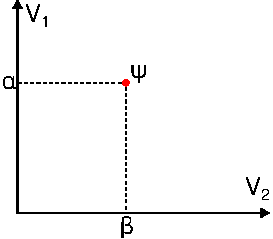
\includegraphics{images/diracPlot}
				\caption{Visual representation of Equation \ref{eq:ketNotationGeneric}. Vectors $V_1$ and $V_2$ must be orthogonal and normalized.}
				\label{fig:diracPlot}
			\end{figure}
	
			\par In quantum mechanics, a state can be represented by different levels depending on the system. For instance, the previous example illustrated a representation of a \textbf{two-level state system}. However, it is important to note that a state can be extended to include one, two, or even multiple levels ($n$).\newline
			
			\par To represent multiple-level states, a common approach is to utilize a vector space with a basis that corresponds to the distinct levels of the system. Each level is associated with a specific vector in the vector space.\newline
			
			\par For instance, consider a three-level system. We can define a basis as ${\ket{V_0}, \ket{V_1}, \ket{V_2}}$, where $\ket{V_0}$, $\ket{V_1}$, and $\ket{V_2}$ represent the vectors associated with the respective levels.
			
			\par In general, a state in a multiple-level system can be expressed as a linear combination of these basis vectors:
			
			\begin{equation}
				\ket{\psi} = \alpha \ket{V_0} + \beta \ket{V_1} + \gamma \ket{V_2} \qquad,
				\label{eq:multipleLevelState}
			\end{equation}
		
			\par Here, $\alpha$, $\beta$, and $\gamma$ are complex coefficients that determine the \textbf{amplitudes} of the state in each level.\newline
			
			\par Being $N=$ the number of levels and $a \in (\alpha, \beta, \gamma, \dots , \omega)$ sometimes the equation \ref{eq:multipleLevelState} can be represented as a sum:
			
			\begin{equation}
				\ket{\psi} = \sum_{i=1}^{N} a_i . \ket{V_i}= 
				\begin{bmatrix}
					a_{1} \\
					a_{2} \\
					\vdots \\
					a_{n}
				\end{bmatrix}
				\label{eq:multipleLevelStateSum}
			\end{equation}
		
			\par Some authors prefers to use $\ket{0}, \ket{1}, \ket{2}, \dots , \ket{n} / n < N$ instead of $\ket{V_0},\ket{V_1}, \dots, \ket{V_n} / n < N$.\newline

			\par Note that this representation is nothing more than another way of defining a \textbf{vector} considering a \textbf{vector space basis} already used in linear algebra, as shown in Equation \ref{eq:linearCombination}!\newline
			
			\begin{equation}
				\label{eq:linearCombination}
				\begin{aligned}
					\ket{\psi} =
					\begin{bmatrix}
						a_{1} \\
						a_{2} \\
						\vdots \\
						a_{n}
					\end{bmatrix} =
					a_1 . \begin{bmatrix}
						1\\
						0\\
						\vdots \\
						0
					\end{bmatrix}+
					a_2 . \begin{bmatrix}
						0\\
						1\\
						\vdots \\
						0
					\end{bmatrix}+
					\dots + a_n . \begin{bmatrix}
						0\\
						0\\
						\vdots \\
						1
					\end{bmatrix}
				\end{aligned}
			\end{equation}
		
			\par Remember this basis vectors $
			\begin{bmatrix}
				1\\
				0\\
				\vdots \\
				0
			\end{bmatrix}, 
			\begin{bmatrix}
				0\\
				1\\
				\vdots \\
				0
			\end{bmatrix}, \dots,
			\begin{bmatrix}
				0\\
				0\\
				\vdots \\
				1
			\end{bmatrix}$ are the \textbf{system possible states}!
		
		\subsection{Probability amplitude}
			\label{sec:probAmpli}
			\par As shown in a previous section, the probability amplitudes represented by the values $[a_1,a_2,a_3, \dots, a_n]$ reside in the complex number set $\mathbb{C}$. In some cases, $a_n$ may have a value in the format $u + vi$, where $u, v \in \mathbb{R}$ and $i = \sqrt{-1}$, indicating a number that is \textbf{not real}. Therefore, in this context, it is not possible to assign a meaningful interpretation to these numbers.\newline
			
			\par To address this issue, we need to introduce the concept of the complex conjugate of a number. For a number $z = u + vi$, where $z \in \mathbb{C}$, its conjugate is denoted as $z^*$, where $z^* \in \mathbb{C}$, and it is given by $z^* = u - vi$. In summary, if $z = u + vi$, then $z^* = u - vi$. \newline
			
			\par By applying the concept of the complex conjugate, we can see that $z \cdot z^* = (u + vi) \cdot (u - vi) = u^2 + v^2 \in \mathbb{R}$. This resolves the problem, as the product $z \cdot z^*$ is a real number!\newline
			
			\par Finally, let \(P(S_i)\) be a function that calculates the probability of the state \(S_i\) occurring. For instance, if \(|\psi\rangle = \alpha |S_0\rangle + \beta |S_1\rangle\), then \(P(S_0)\) and \(P(S_1)\) are defined as shown in equations \ref{eq:state0} and \ref{eq:state1} \cite{binney2013physics}.
			
			\begin{equation}
				\label{eq:state0}
				P(S_0) = \alpha . \alpha^* 
			\end{equation} 
			
			\begin{equation}
				\label{eq:state1}
				P(S_1) = \beta . \beta^* 
			\end{equation}

		\subsection{Bra notation}
			\label{sec:braNotation}
			
			\par Briefly, given a ket $\ket{\psi}$ (as shown in equation \ref{eq:ket}), its corresponding bra is denoted by the conjugate transpose of $\ket{\psi}$ (equation \ref{eq:bra}).
			
			\begin{equation}
				\label{eq:ket}
				\ket{\psi} = 
				\begin{bmatrix}
					u + vo \\
					k + ji \\
					o + li \\
					d + mi
				\end{bmatrix} \in \mathbb{C}
			\end{equation}
		
			\begin{equation}
				\label{eq:bra}
				\bra{\psi} = [u - vo, k - ji, o - li, d - mi]
			\end{equation}
		
			\par When calculating the probability of a specific state, as discussed in section \ref{sec:probAmpli}, a new question arises: \textit{What if there is a need to calculate the total probability of all possible states?} This is where the "bra" notation comes into play!\newline
			
			\par As we already know, a vector of all probability amplitudes, denoted as $\bra{\psi}$, is given by equation \ref{eq:multipleLevelStateKet}. So, for these "ket" states, there is an associated "bra" notation defined in equation \ref{eq:multipleLevelStateBra} \cite{notacaoDirac}
			
			\begin{equation}
				\ket{\psi} = \sum_{i=1}^{N} a_i . \ket{V_i} = 
				\begin{bmatrix}
					a_{1} \\
					a_{2} \\
					\vdots \\
					a_{n}
				\end{bmatrix}
				\label{eq:multipleLevelStateKet}
			\end{equation}
			
			\begin{equation}
				\bra{\psi} = \sum_{j=1}^{N} a_j^* . \bra{V_j} = [a_1^*, a_2^*, \dots, a_n^*]
				\label{eq:multipleLevelStateBra}
			\end{equation}				
			
			\par Considering the equations \ref{eq:multipleLevelStateKet} and \ref{eq:multipleLevelStateBra}, it is now possible, based on what was discussed in section \ref{sec:probAmpli}, to derive a new equation, denoted as \ref{eq:multipleLevelStateBraKet}. This sum corresponds to the overall probability of the system existing in this particular configuration!
			
			
			\begin{equation}
				\begin{aligned}
					\braket{\psi|\psi} = [a_1^*, a_2^*, \dots, a_n^*] . \begin{bmatrix}
						a_{1} \\
						a_{2} \\
						\vdots \\
						a_{n}
					\end{bmatrix} = &\\ 
					a_1^*.a_1 + a_2^*.a_2 + \dots + a_n^*.a_n = &\\
					P(S_1) + P(S_2) + \dots + P(S_n) = &\\
					\sum_{i=1}^{N} P(S_i)
				\end{aligned}
				\label{eq:multipleLevelStateBraKet}
			\end{equation}
		
			\par Bra notation allows for the calculation of inner products between vectors. The inner product of a bra vector $\bra{\psi}$ and a ket vector $\ket{\phi}$ is denoted as $\braket{\psi|\phi}$. The inner product yields a complex number, providing information about the similarity or overlap between the two vectors.\newline
			
			\par For instance, given a vector 
				$\ket{\alpha}= 
				\begin{bmatrix}
					1 \\
					0
				\end{bmatrix}
				$
				 and 
				 $\ket{\beta} = \begin{bmatrix}
					0\\
					1
				\end{bmatrix}$ 
				using the "BraKet" operators to represent the inner product, it will end up like in equation \ref{eq:braket}.
			
			\begin{equation}
				\label{eq:braket}
				\braket{\alpha|\beta} = 
				[1, 0] .
				\begin{bmatrix}
					0 \\
					1
				\end{bmatrix} = 1.0 + 0.1 = 0
			\end{equation}

	\section{Heisenberg principle}
	
		\par This idea can be explained in the context of analyzing variable signals. The challenge lies in determining both the frequencies and their corresponding locations within the signal.\newline
		
		\par To address this challenge, a tool called the Fourier transformation can be employed. Typically, when analyzing a signal, it is common practice to create a "window," which represents the segment size that will be processed. The largest window encompasses all the values of the signal, while the smallest window contains only one value (in the case of discrete sampling).\newline
		
		\par In Figure \ref{fig:noisysignal}, a multi-frequency signal is depicted. Applying the Fourier transformation to the entire signal enables the discovery of all the frequencies present, but it does not provide information about where these frequencies occur within the signal. On the other hand, using a small window allows us to identify the locations of certain high-frequency signal components, but it hinders our ability to determine the locations of lower frequencies, as illustrated in Figure \ref{fig:windowednoisysignal}.\newline
		
		\par In short, when it comes to analyzing signals, the size of the window plays a crucial role. A larger window facilitates more accurate frequency measurement but sacrifices the ability to determine their precise locations. Conversely, a smaller window provides better localization but compromises the accuracy of frequency measurements.

	
		\begin{figure}[h]
			\centering
			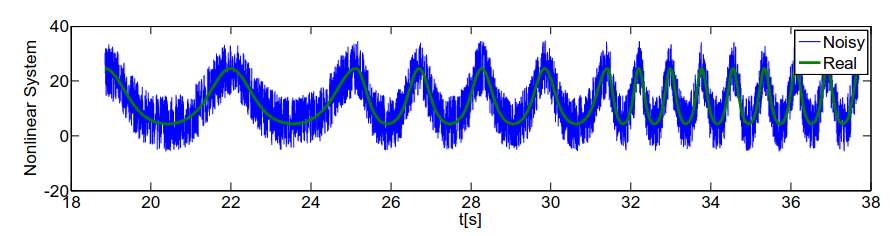
\includegraphics[width=1\linewidth]{images/noisySignal}
			\caption[Multi-frequency signal]{Multi-frequency signal. Source: \cite{olama2011design}}
			\label{fig:noisysignal}
		\end{figure}
		
		
		\begin{figure}[!h]
			\centering
			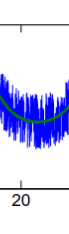
\includegraphics[width=0.1\linewidth]{images/windowedNoisySignal}
			\caption[Windowed signal]{Small windowed signal. Adapted from: \cite{olama2011design}}
			\label{fig:windowednoisysignal}
		\end{figure}

	
	\section{Quantum Bit (Qubit)}
		\par Qubits, unlike classical bits, do not have a defined state and exist in a superposition of states 1 and 0 until they are measured, at which point their state collapses to either 1 or 0 with probabilities given by $|\alpha|^2$ and $|\beta|^2$ respectively, as represented in Equation \ref{eq:qubit} and Figure \ref{fig:qubitplot} \cite{da2018introduccao}.
		
		\begin{equation}
			\ket{\psi} = \alpha . \ket{0} + \beta . \ket{1} = 
			\alpha . \begin{bmatrix}
				1 \\
				0
			\end{bmatrix} + \beta .	\begin{bmatrix}
				0 \\
				1
			\end{bmatrix} = 
			\begin{bmatrix}
				\alpha \\
				\beta
			\end{bmatrix}
			\label{eq:qubit}
		\end{equation}
	
		\par The coefficients $\alpha$ and $\beta$ are complex numbers such that ${|\alpha|}^2 + {|\beta|}^2 = 1$, the vector 
		$\begin{bmatrix}
			\alpha \\
			\beta 
		\end{bmatrix}$ is the qubit itself and, by convention, $\ket{1} = 
		\begin{bmatrix}
			0 \\
			1
		\end{bmatrix} = 1$ and $\ket{0} = 
		\begin{bmatrix}
			1 \\
			0
		\end{bmatrix} = 0$
	
		\begin{figure}[h]
			\centering
			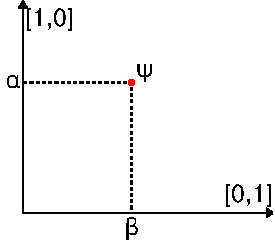
\includegraphics{images/qubitPlot}
			\caption{Visual representation of Equation \ref{eq:qubit}. Vectors $1$ and $2$ must be orthogonal and normalized. $\alpha$ and $\beta$ represent the probabilities associated with the state $\psi$.}
			\label{fig:qubitplot}
		\end{figure}
		
		\par The Equation \ref{eq:qubit} can be interpreted as follows: The \textbf{non-measured} state of $\psi$ within the vector space defined by vectors $\ket{1}$ and $\ket{0}$ is a linear combination of them  ($\alpha$ times vector $\ket{0}$ plus $\beta$ times vector $\ket{1}$).\newline
		
		\par It's important to note that in Figure \ref{fig:qubitplot} and Equation \ref{eq:qubit}, a quantum state is often in a superposition because $\alpha$ and $\beta$ can take on multiple values along the bases axis. For example, if $\alpha = 1$ and $\beta = 0$, the qubit has a $100\%$ probability of being a 0 and $0\%$ probability of being a 1. Conversely, if $\alpha = \frac{1}{\sqrt{2}}$ and $\beta = \frac{1}{\sqrt{2}}$, there is a $50\%$ probability of being 1 and a $50\%$ of being 0.\newline
		
		\par One good example of what a qubit can be is a photon. This particle has electric and magnetic components, forming an electric-magnetic field. We can interpret, for instance, the "vertical" component as the state 0 and the "horizontal" component as the state 1, as depicted in Figure \ref{fig:photonstate01}.
		
		\begin{figure}[H]
			\centering
			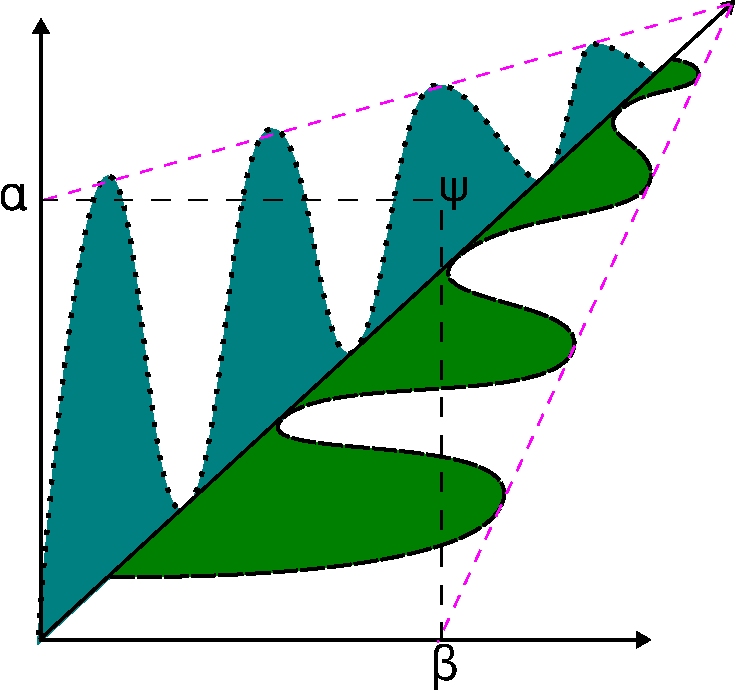
\includegraphics[width=0.5\linewidth]{images/photonState01}
			\caption[Qubit state]{Qubit state: $\alpha$ is the probability of this qubit collapsing to 0, and $\beta$ is the probability of this qubit collapsing to 1.}
			\label{fig:photonstate01}
		\end{figure}
		
		\par Note that in Figure \ref{fig:photonstate01}, there is a \textbf{superposition} of states, meaning that both 0 and 1 values can be assumed when the qubit is measured.\newline
		
		\begin{figure}[H]
			\centering
			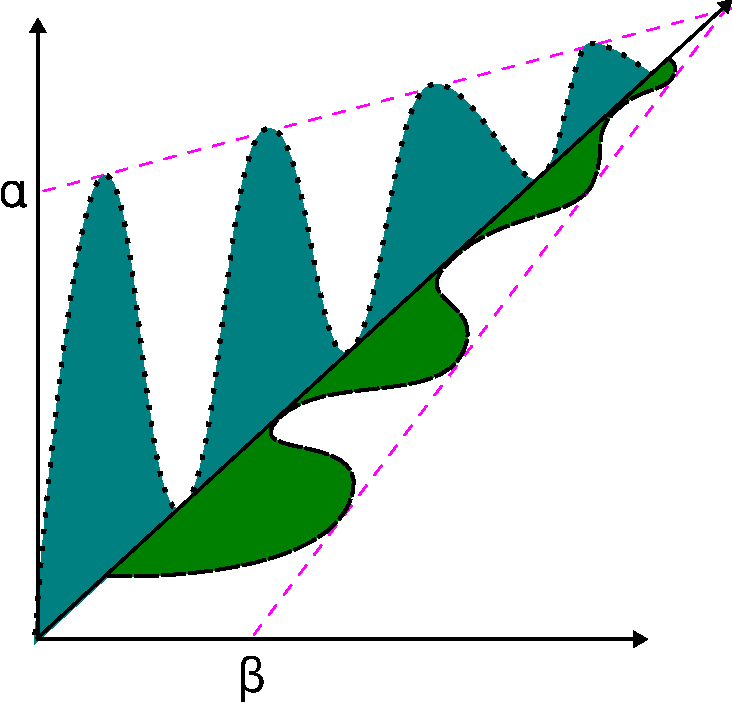
\includegraphics[width=0.5\linewidth]{images/photonState02}
			\caption[Qubit state 2]{Qubit state: $\alpha$ is the probability of this qubit collapsing to 0, and $\beta$ is the probability of this qubit collapsing to 1.}
			\label{fig:photonstate02}
		\end{figure}
		
		\par Note that in Figure \ref{fig:photonstate02}, there is also a \textbf{superposition}, but here the qubit state is more likely to collapse to 0 because of a larger $\alpha$.\newline
		
		\begin{figure}[H]
			\centering
			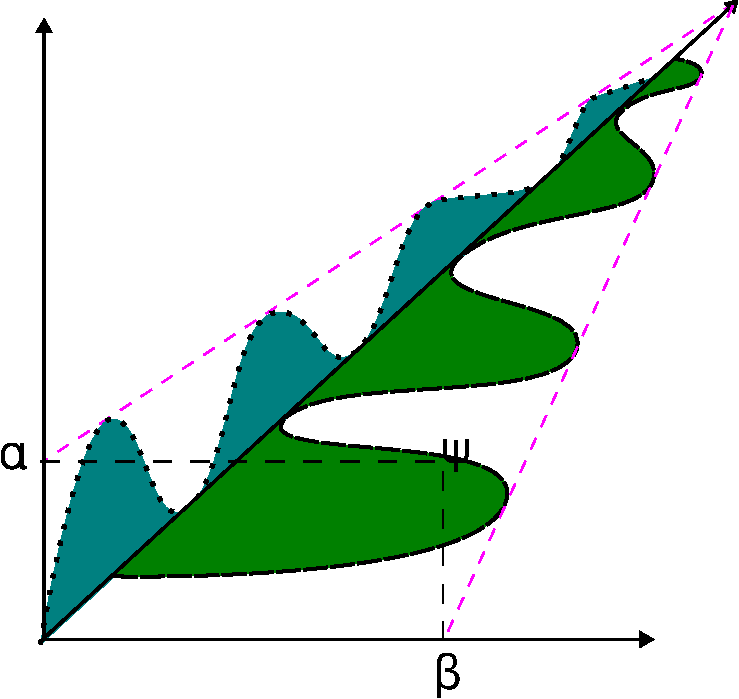
\includegraphics[width=0.5\linewidth]{images/photonState03}
			\caption[Qubit state 3]{Qubit state: $\alpha$ is the probability of this qubit collapsing to 0, and $\beta$ is the probability of this qubit collapsing to 1.}
			\label{fig:photonstate03}
		\end{figure}
		
		\par Again in Figure \ref{fig:photonstate03}, there is a \textbf{superposition}, but note that here the qubit state is more likely to collapse to 1 because of a larger $\beta$.\newline

		\par Qubits have the ability to store and process information differently than classical bits due to superposition. Their capacity, in terms of information storage, is significantly larger compared to classical bits. However, there is a catch: when qubits are measured, they collapse into classical bits. Therefore, currently, it is not possible to take full advantage of the quantum properties for data storage purposes. Furthermore, qubits can store non-binary data, such as $\begin{bmatrix} \dfrac{1}{\sqrt{2}} \\\\ \dfrac{1}{\sqrt{2}} \end{bmatrix}$ or $\begin{bmatrix} \dfrac{1}{2} \\\\ \dfrac{\sqrt{3}}{2} \end{bmatrix}$.\newline
		
		\par Another challenge that arises with systems containing many qubits is decoherence. Due to the limitations of current technology, as the number of qubits increases, so does the presence of noise. This leads to a higher likelihood of random collapses and decoherence between the states of qubits.\newline
		
		\par The List bellow shows the qubits capacity.
		
		\begin{itemize}
			\label{lst:qubits}
			\item 1 qubit = 2 bits
			\item 2 qubits = 4 bits
			\item 3 qubits = 8 bits (1 byte)
			\item 4 qubits = 16 bits
			\item 13 qubits = 8,192 bits (1 kilobyte)
			\item 23 qubits = 8,388,608 bits (1 megabyte)
			\item 33 qubits = 8,589,934,592 bits (1 gigabyte)
			\item 43 qubits = 8,796,093,022,208 bits (1 terabyte)
			\item n qubits = $2^n$ bits
		\end{itemize}
	
	
	\section{Quantum operations}
		\label{sec:quantumOperations}
				
		\par The state vector of a quantum system can undergo various quantum operations, including unitary transformations and measurements. These operations enable the modification of the state vector and the extraction of information from it, facilitating the study of system properties and the prediction of measurement outcomes.\newline
		
		\par The Quantum operations gates serve as unitary linear transformations that preserve orthogonality, ensuring that the quantum state remains normalized and the probabilities of different outcomes are preserved.\newline
		
		\par To preserve normalization, quantum gates \textbf{must} satisfy certain conditions. Let $G$ be a matrix representing a quantum gate and $G^*$ its conjugate transpose, and let $I$ be an identity matrix. A gate $G$ must be unitary being $G \cdot G^* = I$ \cite{da2018introduccao}.
		
		\subsection{Quantum gates}
		
			\par As mentioned earlier, quantum gates are represented as matrices, and their number is infinite because the values of the matrix cells can vary across the real numbers ($\mathbb{R}$). Although there is a wide variety of quantum gates and considering $\ket{\psi} = \alpha . \ket{0} + \beta . \ket{1}$, here are a few examples.\newline

		
			\par The \textbf{identity gate} in Equation \ref{eq:indentity} alters the qubit state as shown in Equation \ref{eq:indentityApplyed}.
			\begin{equation}
				\label{eq:indentity}
					I : 
					\begin{bmatrix}
						1& 0 \\
						0& 1
					\end{bmatrix}
			\end{equation}

			\begin{equation}
				\label{eq:indentityApplyed}
				I\ket{\psi} = \begin{bmatrix}
					1& 0 \\
					0& 1
				\end{bmatrix} . \begin{bmatrix}
					\alpha \\
					\beta
				\end{bmatrix} = \begin{bmatrix}
					\alpha \\
					\beta
				\end{bmatrix} = \ket{\psi}
			\end{equation}
		
			\par The \textbf{flip gate} in Equation \ref{eq:flip} flips the qubit state as shown in Equation \ref{eq:indentityApplyed}.
			\begin{equation}
				\label{eq:flip}
				X : 
				\begin{bmatrix}
					0& 0 \\
					1& 0
				\end{bmatrix}
			\end{equation}
			
			\begin{equation}
				\label{eq:flipApplyed}
				X\ket{\psi} = \begin{bmatrix}
					0& 1 \\
					1& 0
				\end{bmatrix} . \begin{bmatrix}
					\alpha \\
					\beta
				\end{bmatrix} = \begin{bmatrix}
					\beta \\
					\alpha
				\end{bmatrix}
			\end{equation}
		
		
			\par The \textbf{Hadamard gate} in Equation \ref{eq:hadamard} puts the qubit state in to \textbf{superposition} \cite{qcfcs}  with the same probability for the two states \cite{da2018introduccao} allowing as shown in Equation \ref{eq:hadamardApplyed}.
			\begin{equation}
				\label{eq:hadamard}
				H : \dfrac{1}{\sqrt{2}}.
				\begin{bmatrix}
					1& 1 \\
					1& -1
				\end{bmatrix}
			\end{equation}
			
			\begin{equation}
				\label{eq:hadamardApplyed}
				\begin{aligned}
					&H\ket{\psi} = \dfrac{1}{\sqrt{2}}.\begin{bmatrix}
						1& 1 \\
						1& -1
					\end{bmatrix} . \begin{bmatrix}
						\alpha \\
						\beta
					\end{bmatrix} = \\
					&\begin{bmatrix}
						\dfrac{1}{\sqrt{2}} &\dfrac{1}{\sqrt{2}} \\
						\dfrac{1}{\sqrt{2}} &\dfrac{-1}{\sqrt{2}}
					\end{bmatrix} .
					\begin{bmatrix}
						\alpha \\
						\beta
					\end{bmatrix} = 
					\begin{bmatrix}
						\alpha . \dfrac{1}{\sqrt{2}} + \beta.\dfrac{1}{\sqrt{2}} \\
						\alpha . \dfrac{1}{\sqrt{2}} + \beta.\dfrac{-1}{\sqrt{2}}
					\end{bmatrix} = \\
					&\begin{bmatrix}
						\dfrac{1}{\sqrt{2}} . (\alpha + \beta) \\
						\dfrac{1}{\sqrt{2}} . (\alpha - \beta)
					\end{bmatrix}
				\end{aligned}
			\end{equation}
		
			\par To further illustrate this, let's consider a numeric example. We start with a qubit state $\begin{bmatrix} 1 \\ 0 \end{bmatrix}$, which is not in superposition. We can apply the Hadamard gate to put it into superposition. The resulting state is given by Equation \ref{eq:hadamardApplyedNum}.
			
			\begin{equation}
				\label{eq:hadamardApplyedNum}
				\begin{aligned}
					&H\ket{\psi} = \dfrac{1}{\sqrt{2}}.\begin{bmatrix}
						1& 1 \\
						1& -1
					\end{bmatrix} . \begin{bmatrix}
						1 \\
						0
					\end{bmatrix} = \\
					&\begin{bmatrix}
						\dfrac{1}{\sqrt{2}} &\dfrac{1}{\sqrt{2}} \\
						\dfrac{1}{\sqrt{2}} &\dfrac{-1}{\sqrt{2}}
					\end{bmatrix} .
					\begin{bmatrix}
						1 \\
						0
					\end{bmatrix} = 
					\begin{bmatrix}
						1 . \dfrac{1}{\sqrt{2}} + 0.\dfrac{1}{\sqrt{2}} \\
						1 . \dfrac{1}{\sqrt{2}} + 0.\dfrac{-1}{\sqrt{2}}
					\end{bmatrix} = \\
					&\begin{bmatrix}
						\dfrac{1}{\sqrt{2}} . (1 + 0) \\
						\dfrac{1}{\sqrt{2}} . (1 - 0)
					\end{bmatrix} = 
					\begin{bmatrix}
						\dfrac{1}{\sqrt{2}} \\
						\dfrac{1}{\sqrt{2}}
					\end{bmatrix}
				\end{aligned}
			\end{equation}
			
			\par The Hadamard gate possesses another interesting property: when applied to a quantum bit, it can transform it from a superposition state to a classical bit with measurement, i.e. not triggering the collapse. This property makes the Hadamard gate useful for extracting results from quantum algorithms. Furthermore, the Hadamard gate can also perform the opposite operation: it can convert a classical bit into a superposition state. This allows for computation in the quantum realm, and by applying the Hadamard gate again, the results can be extracted from the superposition state \cite{qcfcs}.\newline

			\par The \textbf{rotation gate} in Equation \ref{eq:rot} rotates the qubit state $\pi$ radians as shown in Equation \ref{eq:rotApplyed}.
			\begin{equation}
				\label{eq:rot}
				Z : 
				\begin{bmatrix}
					1& 0 \\
					0& -1
				\end{bmatrix}
			\end{equation}
			
			\begin{equation}
				\label{eq:rotApplyed}
				Z\ket{\psi} = \begin{bmatrix}
					1& 0 \\
					0& -1
				\end{bmatrix} . \begin{bmatrix}
					\alpha \\
					\beta
				\end{bmatrix} = \begin{bmatrix}
					\alpha \\
					-\beta
				\end{bmatrix}
			\end{equation}

			\par The \textbf{conditional not gate}(CNOT) in Equation \ref{eq:cnot} may create an \textbf{entanglement} between two qubits \cite{nielsen2002quantum}.
			\begin{equation}
				\label{eq:cnot}
				CNOT : 
				\begin{bmatrix}
					1& 0& 0& 0 \\
					0& 1& 0& 0 \\
					0& 0& 0& 1 \\
					0& 0& 1& 0
				\end{bmatrix}
			\end{equation}
		
			\par This gate operates on \textbf{two qubits}, where one is the \textbf{control qubit} and the other is the \textbf{target qubit}. To represent the state of the combined qubits, a variation of ket notation is used, where two vectors are represented together. This is necessary because the qubits can no longer be written separately due to the entanglement this gate may cause. The ket variations are shown in Equations \ref{eq:ketForTwoVectors00}, \ref{eq:ketForTwoVectors01} and \ref{eq:ketForTwoVectors02}.
			
			\begin{equation}
				\label{eq:ketForTwoVectors00}
				\ket{1}, \ket{0} \implies
				\ket{10} = \begin{bmatrix}
					0 \\
					1 \\
					1 \\
					0
				\end{bmatrix}				
			\end{equation}
		
			\begin{equation}
				\label{eq:ketForTwoVectors01}
				\ket{0}, \ket{0} \implies
				\ket{00} = \begin{bmatrix}
					1 \\
					0 \\
					1 \\
					0
				\end{bmatrix}				
			\end{equation}
			
			\begin{equation}
				\label{eq:ketForTwoVectors02}
				\ket{1}, \ket{1} \implies
				\ket{11} = \begin{bmatrix}
					0 \\
					1 \\
					0 \\
					1
				\end{bmatrix}				
			\end{equation}
			
			\par The CNOT gate operates on two qubits, where the first qubit serves as the control and the second qubit as the target. As shown in the Equation \ref{eq:cnotApplyed}, when the control qubit is in the state $\ket{1}$, the target qubit undergoes a flip. However, when the control qubit is in the state $\ket{0}$, the target qubit remains unchanged.
			
			\begin{equation}
				\label{eq:cnotApplyed}
				\begin{aligned}
					&CNOT\ket{00} = \ket{00}, \\
					&CNOT\ket{01} = \ket{01}, \\
					&CNOT\ket{10} = \ket{11}, \\
					&CNOT\ket{11} = \ket{10}
				\end{aligned}
			\end{equation}


			\par Please note that, as aforementioned, this is just a sample of the possible gates, and that these ones were selected for their relevance according to the judgment of the author.

	\section{Conclusion}
		\par It is worth noting that all the examples presented in this document intentionally avoided the use of numbers from the complex set $\mathbb{Q}$. This choice was made to facilitate the understanding of the topic. However, if you are interested in delving deeper into the subject, I recommend consulting the provided references and keywords for further reading.
		
		\par This said: That's all folks!	
	\bibliographystyle{plain}
	\bibliography{references.bib}
\end{document}